%-----------------------------------------------------------------------------
%
%               Template for sigplanconf LaTeX Class
%
% Name:         sigplanconf-template.tex
%
% Purpose:      A template for sigplanconf.cls, which is a LaTeX 2e class
%               file for SIGPLAN conference proceedings.
%
% Guide:        Refer to "Author's Guide to the ACM SIGPLAN Class,"
%               sigplanconf-guide.pdf
%
% Author:       Paul C. Anagnostopoulos
%               Windfall Software
%               978 371-2316
%               paul@windfall.com
%
% Created:      15 February 2005
%
%-----------------------------------------------------------------------------


\documentclass{sigplanconf}

% The following \documentclass options may be useful:

% preprint      % Remove this option only once the paper is in final form.
% 10pt          To set in 10-point type instead of 9-point.
% 11pt          To set in 11-point type instead of 9-point.
% authoryear    To obtain author/year citation style instead of numeric.

\usepackage{amsmath}
\usepackage{natbib}
\usepackage{graphicx}
\usepackage{wrapfig}
\usepackage{caption}


\begin{document}

\special{papersize=8.5in,11in}
\setlength{\pdfpageheight}{\paperheight}
\setlength{\pdfpagewidth}{\paperwidth}

\conferenceinfo{CONF 'yy}{Month d--d, 20yy, City, ST, Country} 
\copyrightyear{20yy} 
\copyrightdata{978-1-nnnn-nnnn-n/yy/mm} 
\doi{nnnnnnn.nnnnnnn}

% Uncomment one of the following two, if you are not going for the 
% traditional copyright transfer agreement.

%\exclusivelicense                % ACM gets exclusive license to publish, 
                                  % you retain copyright

\permissiontopublish             % ACM gets nonexclusive license to publish
                                  % (paid open-access papers, 
                                  % short abstracts)

\titlebanner{banner above paper title}        % These are ignored unless
\preprintfooter{short description of paper}   % 'preprint' option specified.

\newcommand{\pname}{KinEdit}

\title{\pname{}}
\subtitle{View and edit all contexts referring to a common identifier}

\authorinfo{Josh Terrell}
           {California Polytechnic University, San Luis Obispo}
           {jmterrel@calpoly.edu}
% \authorinfo{Name2\and Name3}
%            {Affiliation2/3}
%            {Email2/3}

\maketitle

\begin{abstract}
Some developers do not trust automated refactoring tools to refactor correctly.
Without using refactoring tools, refactoring can take longer and result
in more bugs. Developers do not have to trust automated refactoring tools to
take advantage of some productive features that refactoring tools offer.
Using \pname{}, developers can refactor more quickly, with higher
quality, and without needing to trust automated refactoring tools.
% problem. why propblem is problem. startling sentence (make claim). implication.
\end{abstract}

\category{not sure what to put here..CR-number}{subcategory}{third-level}

% general terms are not compulsory anymore, 
% you may leave them out
% \terms
% term1, term2

\keywords
refactoring, tool, trust

\section{Problem and Motivation}
Refactoring is the process of changing the structure of code without changing
its behavior; the goal is to make code more maintainable \cite{legacy-code}.
Studies have shown that refactoring actually can make code more maintainable
\cite{maintainability}. When refactoring, developers may often have the
ability to use an automated refactoring tool to refactor correclty and quickly.
However even though automated refactoring tools exist, some developers continue
to refactor manually. Manual refactoring can be an error prone process
\cite{bene-factor}.

Research shows that software developers do not use automatic software
refactoring tools as often as the tools may be useful \cite{how-refactor}.
\textit{Awareness}, \textit{opportunity}, and
\textit{trust} have been observed to be three reasons for why developers do not
use these tools often \cite{how-refactor, say-refactor}. Awareness refers to
knowing that a tool exists, and opportunity means realizing that one is at an
appropriate circumstance to use a refactoring tool \cite{how-refactor}.

Developers who do not trust automated refactoring
tools may know about the tools, but they do not trust the tools to refactor code
correctly. Some worry that refactoring tools may introduce bugs; others
are concerned with the readability and design of the code produced by the
tools \cite{say-refactor}.
Rather than use the tool, the developers choose to manualy refactor.

When not using an automated refactoring tool, some developers use a technique
called \textit{lean on the compiler} to refactor
code \cite{legacy-code, how-refactor}. Using \textit{lean on the compiler},
developers choosing to, for example, rename a method, first rename the method
declaration to something obscure. The result
is a bunch of errors scattered throughout the code. The developers subsequently
visit these errors, determine a better name for the method using the calling
contexts, rename all references to the method, and finally rename the
declaration.

This method is fairly common in practice\cite{1}, but it is slower and more
error prone than automated refactorings. Still, developers potentially 
wisely choose to continue leaning on the compiler in some refactorings.
They continue to manully iterate through possibly hundreds of errors
clicking on error after error to open and close window after window.

\section{Background and Related Work}
BeneFactor \cite{bene-factor} and WitchDoctor \cite{witch-doctor} are solutions
which both help increase the usage of refactoring tools by increasing 
developers' awareness of refactoring tools. These tools allow developers 
to take more opportunities to use refactoring tools by
detecting when a refactoring is occuring and
allow automatic completion of the refactoring from the current snapshot of code
\cite{bene-factor, witch-doctor}.

GhostFactor takes a different apporach. GhostFactor tackles both the
\textit{awareness} and \textit{trust} reasons by (1) automatically detecting
when a developer has completed a manual refactoring and (2) not
interferring with the developer's manual
refactorings, but instead validating that the developer has refactored
correctly \cite{ghost-factor}.

In contrast to these approcaches, \pname{} does not refactor
for developers nor even have the ability to refactor. Rather, \pname{} simply
provides a
convinient and familiar interface for developers to perform refactorings in
thier own workflow.

\section{Approach and Uniqueness}
\pname{} aids developers who refactor but do not trust
automated refactoring tools. \pname{} does so by allowing
developers to view and edit a refactoring's \textit{touch points}:
the set of places in the code that may be affected by a potential change
\cite{how-refactor}. The goal of this tool is to support
developers' refactoring workflows without requiring them to use tools they do
not trust and interfaces they are not familiar with.

As one example of \pname{} in action, \pname{} can be used to increase the
productivity of a developer performing a \textit{lean on the compiler} refactoring.
\pname{} steps in where the developer visits all the errors scattered througout
the code. With this tool, the developer can bring up Eclipse's Quick Fix for
any error and then choose to open all related errors in another tab.
\begin{center}
\caption*{Fig 1: Rename a method to something obscure to the find callers.}
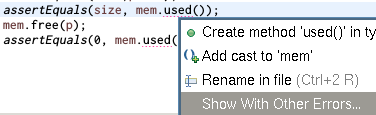
\includegraphics[width=0.35\textwidth]{quick-fix.png}
\end{center}

In the example, the developer wishes to rename the method
\textit{getValidMoves}, so he renames
it to something obscure. He then brings up the quick fix menu of the method
itself (Ctrl+1) or any of the newly created errors and selects
"Show With Other Errors..."

ErrorView subsequently displays a window containing a collection of
editors---each having
one of the related errors in focus. This multiple-editor window allows the
developer to simultaneously view the error
contexts to determine a more suitable method name. Then the developer may make
the desired renaming changes without needing to manually iterate through the
process of opening a new window for each error.
\begin{center}
\caption*{Fig 2: Related errors are each opened in their own editor.}
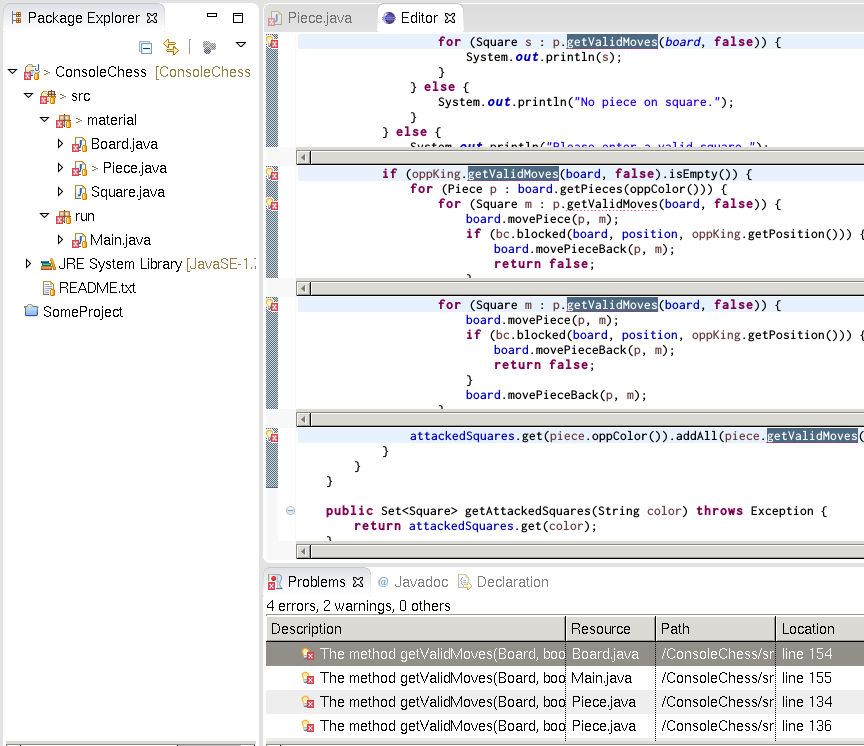
\includegraphics[width=0.50\textwidth]{multiple-editors.png}
\end{center}

The image shows each of the four related errors open and displayed in their own
editor. The developer may now easily and quickly see all the contexts together,
choose an appropriate name, and complete the renaming of the method.

The example above, in comparision to other refactorings,  is a rather trivial
rename refactoring. As it stands,
\pname{} can also help with many other common refactorings.
To name a few, \pname{} can assist developers in performing the refactorings
\textit{pull up/down method}, \textit{add parameter},
\textit{change return type}, and \textit{extract interface}
while giving the developer complete control and a familiar interface.

Currently \pname{} has limited functionality, however it has potential to expand
into a more productive tool. \pname{} currently encompasses one primary
feature---opening a window containing each of a given error's related errors
(including iteself). In the future the tool should have some additional
capabilities:

\begin{itemize}
  \item Right click an identifier to open all references to the method, class,
      or variable in the multiple editor window.
  \item In Eclipse's find all references, include a button on the interface
      to open the multiple-editor window.
  \item Provide a listing in Eclipse's Quick Assist (Ctrl+2).
\end{itemize}


\section{Results and Contributions}
Results, results, results, results. Results, results, results.
Results, results, results, results. Results, results, results.
Results, results, results, results. Results, results, results.
Results, results, results, results. Results, results, results.
Results, results, results, results. Results, results, results.
Results, results, results, results. Results, results, results.
Results, results, results, results. Results, results, results.
Results, results, results, results. Results, results, results.

Results, results, results, results. 
Results, results, results, results. Results, results, results.
Results, results, results, results. Results, results, results.
Results, results, results, results. Results, results, results.

\appendix
% \section{Appendix Title}
% 
% This is the text of the appendix, if you need one.

\acks
Thank you Dr. Emerson Murphy-Hill for your guidance through writing this
paper during my summer research internship at North Carolina State University.
I am also very appreciative of the National Science Foundation which made this
research opportunity and many like it possible.

% We recommend abbrvnat bibliography style.

\bibliographystyle{abbrvnat}

% The bibliography should be embedded for final submission.

\softraggedright
\bibliography{error-view}

\end{document}
